\documentclass{article}
\usepackage[margin=24mm]{geometry}
\usepackage{tikz}
\setlength{\emergencystretch}{3em}
\title{Canonical six-bit inverse composition}
\date{Created-at: 2026-10-28 20:53 CET}
\begin{document}\maketitle
\paragraph{Acceptance.} Synthesize the GF(64) tower inverse, with zero mapped
to zero, from own HyMeKo norm, GF(8) inverse and multiplication specifications.
Preserve the full arbitrary-target XOR contract, input, phase and clean workspace.
Compare separate-output and in-place sub-inverse schedules, and independently
check a public arbitrary-target reference in the same tower coordinates. No full
DQI replacement, Kaggle upload, optimality or RL claim.
\paragraph{Ownership and architecture.} Core/Query retain the canonical model.
Graph's existing local executable supplies source-bound matroid certificates.
Quantum compiles quadratic components, lowers a bounded three-bit involution
from its truth function, and composes typed call/binding hyperedges. The existing
gate emitter and QuantumModel reader own the flattened circuit. Add an explicit
Boolean-permutation execution profile: at most 24 total / 12 data qubits and
512 X/CNOT/Toffoli gates. Reuse one primitive basis-transition implementation;
enumerate at most 4096 valid basis states without dense amplitudes. Existing
unitary limits stay 9 qubits / 64 gates. Dense probe/execute reject larger widths;
probe becomes fallible. Entropy is explicitly unavailable for the sparse profile.
\paragraph{Changes.} Extend Quantum model/simulation/resource/emitter APIs and
quadratic-root selection; add arithmetic composition, metadata, fixture and
focused tests. Reuse Python quadratic authoring and introduce a shared native
reversible-gate adapter, without copying the existing lowering. Extend the
existing Kaggle tool/report workflow. No Graph/Nagare edits or dependency changes.
Protected items: none. Preserve unrelated dirty work; no commit or publication.
\paragraph{Math and schedules.} For x=a+b*y with y*y+y+1=0, compute
N=a*a+a*b+b*b, invert N over GF(8), then accumulate (a+b)/N and b/N into
the two target halves. Reverse every temporary computation. An in-place GF(8)
inverse can be lowered from disjoint transpositions and save three qubits.
Compare complete Q-squared-Toffoli proxy costs; nonlinear workspace costs are
not summed from individual calls. Components and their bindings remain in Core.
\paragraph{Verification.} Check all 4096 input/target states, including zero,
phase and scratch cleanup, using independent native finite-field arithmetic.
Test wrong/foreign witnesses, malformed bindings, unsupported large-profile
operators, dirty cleanup, dense allocation refusal and original profile limits.
The sparse verifier's exact permutation comparison covers the clean input
subspace; no dense-state entropy is fabricated. Existing phase/norm tests remain.
\paragraph{Budget, provenance and ETA.} Freshly fetched Transformation at
32c6bb3, current with upstream. One CPU, 2 GiB hard / 1800 MiB sampled memory,
900 seconds per explicit native check on Amaterasu; no WSL. Existing Graph
binary is an explicit local integration aid, with hash and checked coefficients.
No clean-clone claim. ETA about 60--90 minutes including focused checks, report
and archive. Final verification uses serialized artifacts. Report once, archive
once after writers stop; retain the earlier 883-qubit incumbent.
\paragraph{Risks.} Classical permutations require a separate guarded execution
profile, not a larger unconstrained state vector. A better workspace schedule
need not beat a measurement-assisted reference in Toffoli count. All comparisons
must use identical input/output/zero contracts. Roll back only named task edits.
\paragraph{Measured-cleanup continuation, 21:25 CET.} The unitary own inverse
passes all 4096 basis states at Q15/T30; public iso20 passes at Q18/T20.
Add an explicitly authored inverse-norm erasure macro. Certify the selected
unitary prefix on all 4096 states, including its exact remaining scratch value.
Measure the inverse norm, recompute the norm, repay the inverse polynomial's
classical-mask phase, then measure the norm and repay its quadratic phase from
the original inputs. Check all 64 input words and 8-by-8 measurement masks.
The native schema becomes arithmetic.v2 for this optional lowering; the retained
unitary reference remains in Core. Classical phase corrections use only degree
one/two functions, so the expected cleanup costs 6 instead of 9 Toffolis.
The native instruction cap is 1024, with the original circuit/width bounds
unchanged. Native measurement verification uses three seeds. No speculative
replacement is accepted before both the symbolic and native gates pass.
\paragraph{Outcome.} The measured variant passed all 4096 input/target states
at three measurement seeds, with zero value, phase, round-trip and workspace
errors. Q15/T27 gives proxy 6075 versus public Q18/T20 at 6480 and Q21/T19
at 8379. The existing native selector now also accepts the generic
\texttt{reversible\_kernel} scope under the same strict microkernel contract
checks. 62 targeted Rust and 6 Python tests pass. The native computation moved
to isolated /dev/shm after /home filled; outputs were copied and hashed locally.
No data was deleted to make space, and no complete decoder was replaced.
\begin{center}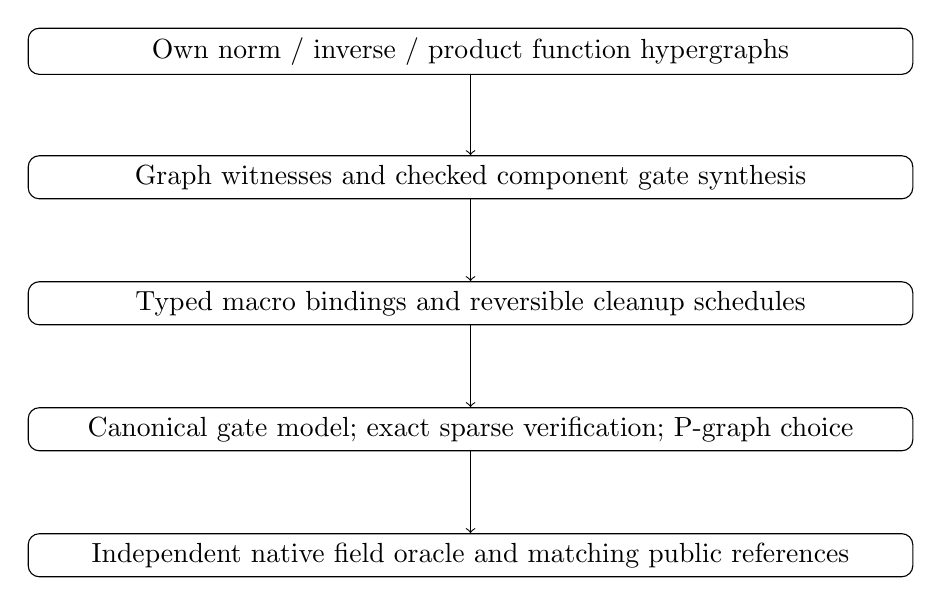
\begin{tikzpicture}[every node/.style={draw,rounded corners,align=center,text width=11cm},node distance=16mm]
\node (a) {Own norm / inverse / product function hypergraphs};
\node (b) [below of=a] {Graph witnesses and checked component gate synthesis};
\node (c) [below of=b] {Typed macro bindings and reversible cleanup schedules};
\node (d) [below of=c] {Canonical gate model; exact sparse verification; P-graph choice};
\node (e) [below of=d] {Independent native field oracle and matching public references};
\draw[->] (a)--(b);\draw[->] (b)--(c);\draw[->] (c)--(d);\draw[->] (d)--(e);
\end{tikzpicture}
\end{center}
\end{document}
